\section{Data Understanding}

The dataset contains \emph{471910} entries, each of them represent a purchase related to a supermarket made by a customer over a period of two years.

\subsection{Data Semantics}

The dataset contains 8 attributes that correspond to:

\begin{itemize}
\item \textbf{BasketID} (\emph{24627}): a 6 digit integer number uniquely assigned to each purchase; if it starts with a \emph{C}, it indicates a cancellation (\emph{3754});
\item \textbf{BasketDate}: the day (\emph{from 2010/12/01 to 2011/12/09}) and time (\emph{from 6am to 21pm}) when each purchase was placed;
\item \textbf{Sale} (\emph{∼4avg}): the unit product price, all in the same currency, probably in sterling;
\item \textbf{CustomerID} (\emph{4372 + 65073na}): a 5 digit integer number uniquely assigned to each customer;
\item \textbf{CustomerCountry} (\emph{37}): the name of the country where each customer resides;
\item \textbf{ProdID} (\emph{3953}): a 5 digit + 1 letter identifier uniquely assigned to each distinct product; identical codes with different letters identify the same products with different characteristics (\emph{e.g.}, \emph{84997D}: '\emph{pink piece polkadot cutlery set} vs. \emph{84997C}: '\emph{blue piece polkadot cutlery set});
\item \textbf{ProdDescr} (\emph{4097 + 753na}): the description of the product purchased;
\item \textbf{Qta} (\emph{∼11avg}): the purchased quantities of each product per order.
\end{itemize}

\subsection{Assessing Data Quality}

In order to assess the quality of data, we proceed by removing the \emph{5232} duplicate entries which represents the 1.11\% of the entire dataset, so we will work with the remaining \emph{466678} rows.

Then, we proceed by removing the entries corresponding to the \emph{65073} null \emph{CustomerID} values, the 13.94\% of the dataset, since there is no way to integrate them to trace the customer's orders.

Afterwards, we removed the \emph{ProdID} that does not respect the defined format and we found some that contains only letters, \emph{e.g.}, '\emph{POST}', '\emph{D}', '\emph{C2}', '\emph{M}', '\emph{BANK CHARGES}', etc. with the following respective \emph{ProdDescr}: '\emph{POSTAGE}', '\emph{Discount}', '\emph{CARRIAGE}', '\emph{Manual}', '\emph{Bank Charges}', etc.

\subsection{Variables Transformations}

\begin{figure}
\centering
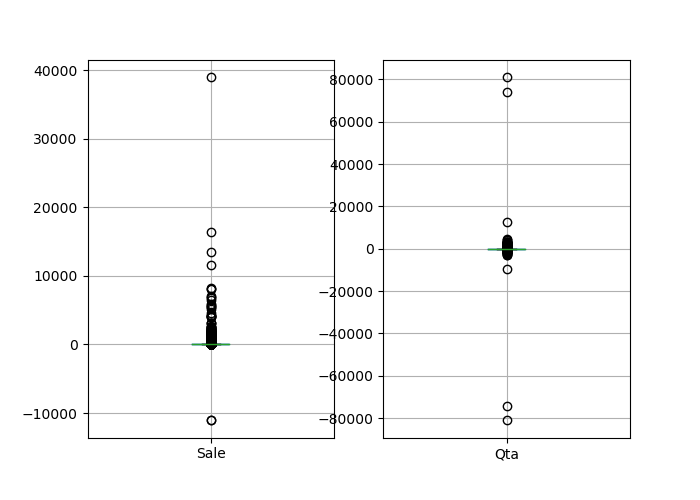
\includegraphics[width=0.49\textwidth]{img/boxplot_before.png}
\caption{\emph{Sale} and \emph{Qta} boxplots}
\label{fig:original_sale_qta_boxplots}
\end{figure}

In order to manage the presence of negative quantities as shown in the boxplot in Figure \ref{fig:original_sale_qta_boxplots}, we decide to keep track of the portion of each order that has been canceled. At this point we should face three different cases:

\begin{itemize}
\item a \emph{cancelation exists with a counterpart}, i.e., exists an order with the same (but positive) quantity and a previous date, so both are canceled;
\item a \emph{cancelation exists without a counterpart}, this is probably due to the fact that the orders were performed before December 2010 (the entry point of the database), so we remove this;
\item a \emph{cancelation exists with multiple counterparts}, so we delete the most recent.
\end{itemize}

To also manage the presence of prices equal to zero as shown in the boxplot in Figure \ref{fig:original_sale_qta_boxplots}, we filled these values with the average of the selling prices of the products with the same id.

We decided to create the attribute \emph{TotSale}, i.e., the product between \emph{Sale} and \emph{Qta}, that represents the total amount spent by a customer for each type of product purchased. We made this choice mainly to have a clearer look to the dataset, emphasizing an important information that was not explicit in the original table, and also for the feature extraction later.

\subsection{Variables Distribution}

\begin{figure}[!h]
\begin{subfigure}{.5\textwidth}
\centering
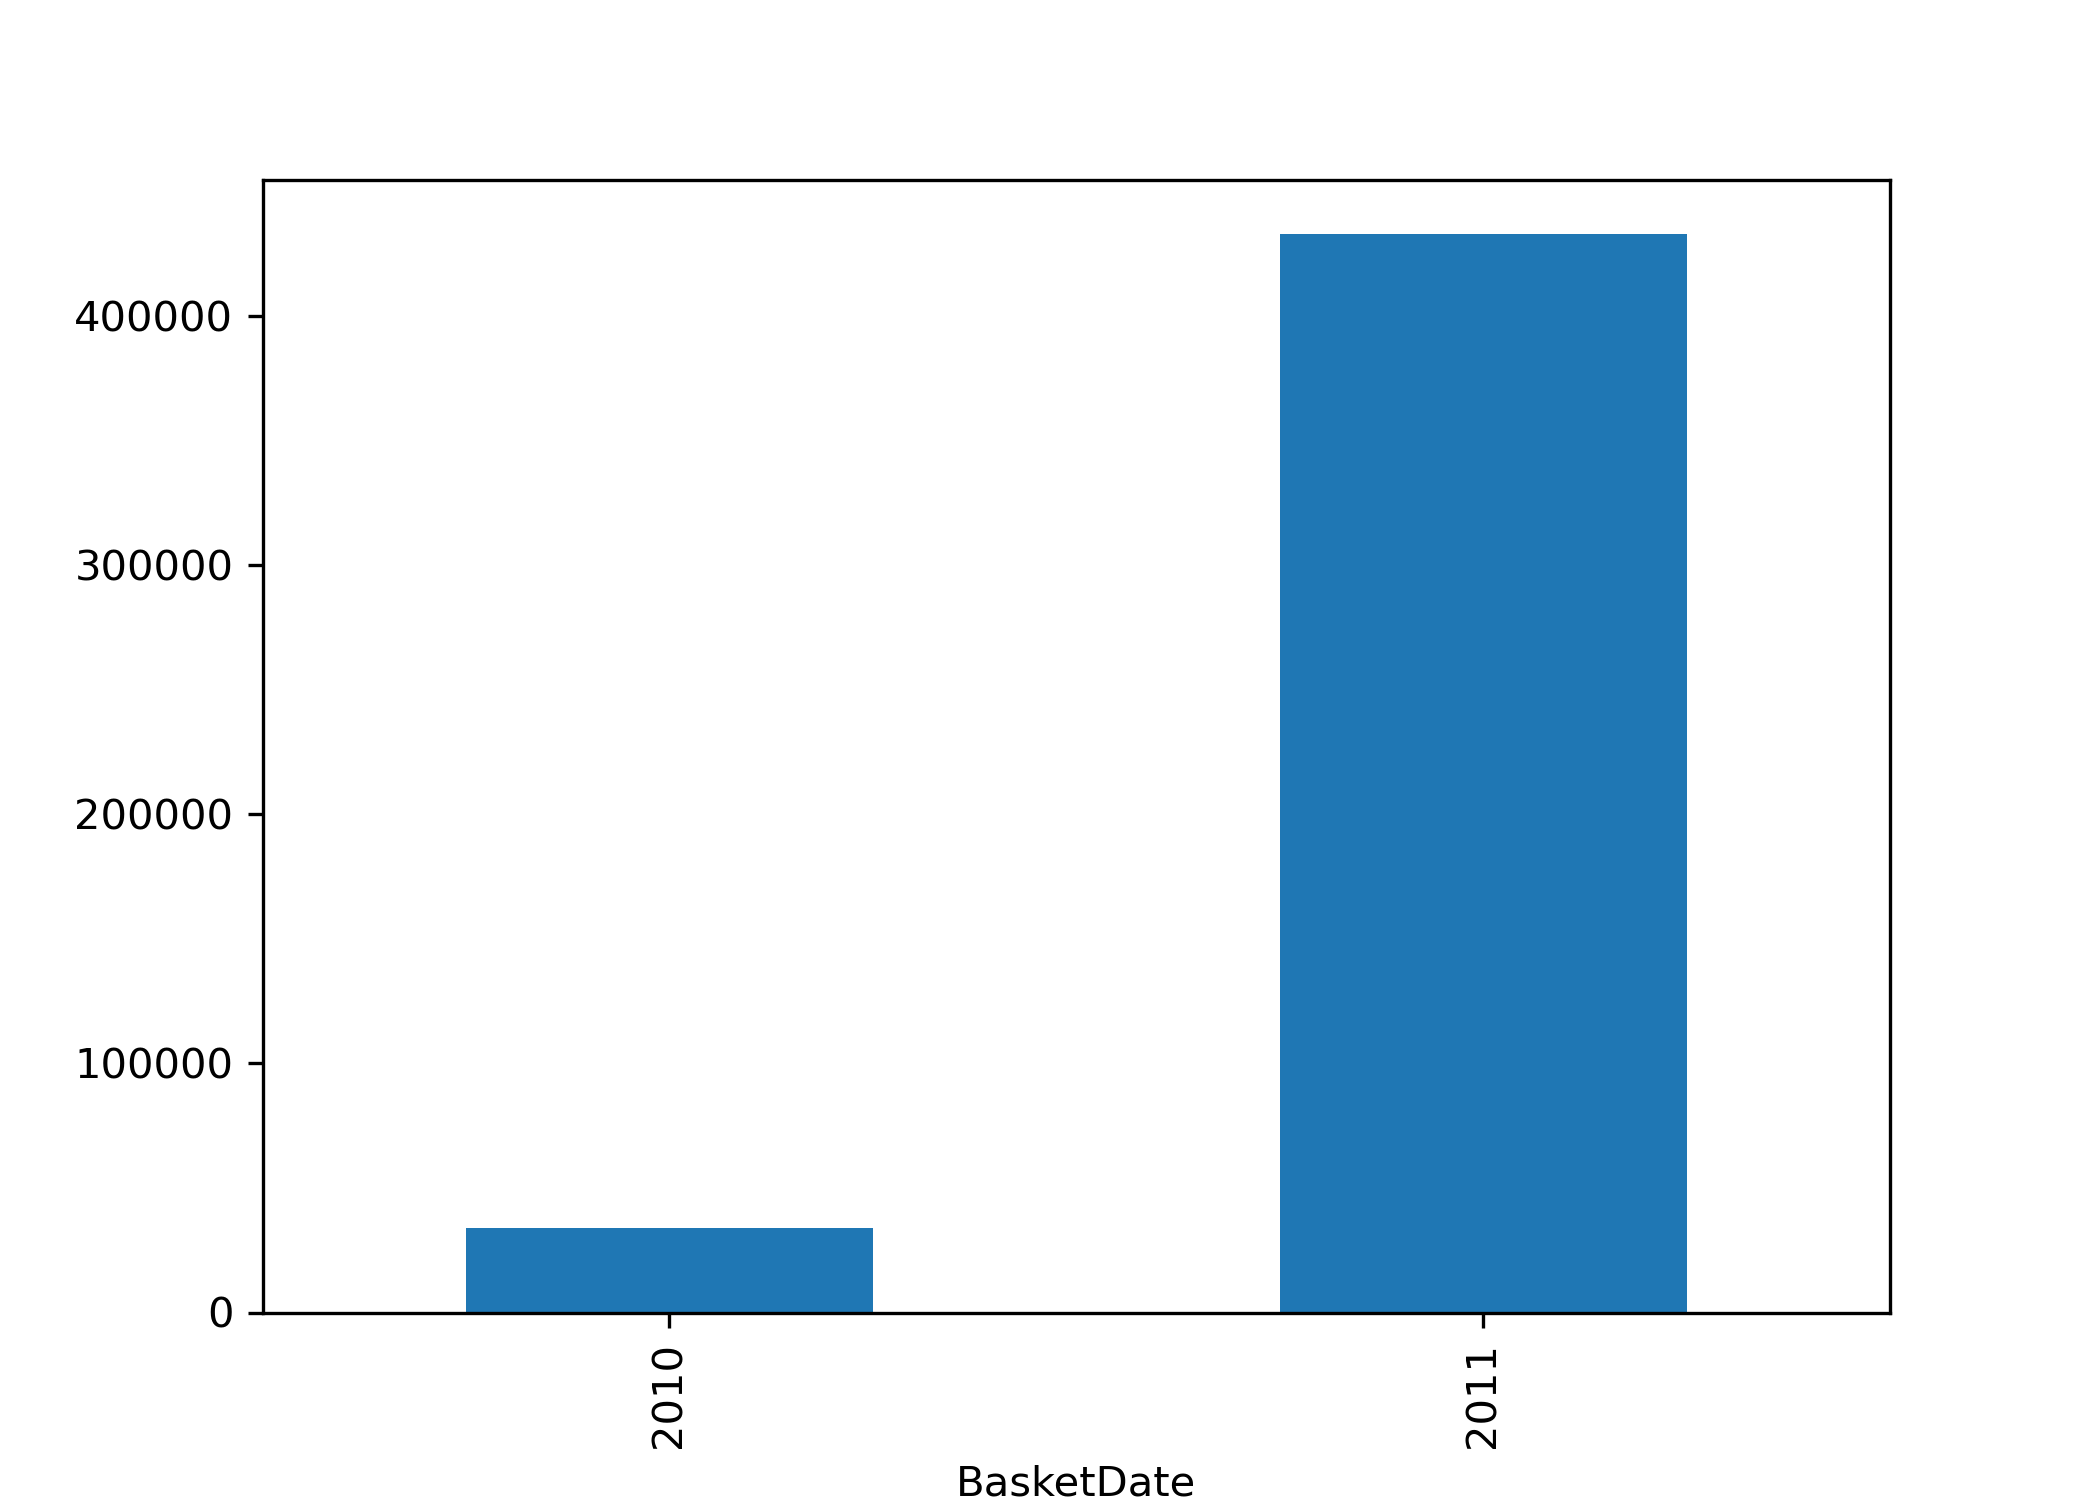
\includegraphics[width=.7\textwidth]{img/year_bar.png}
\caption{Year}
\label{fig:year_bar}
\end{subfigure}
\begin{subfigure}{.5\textwidth}
\centering
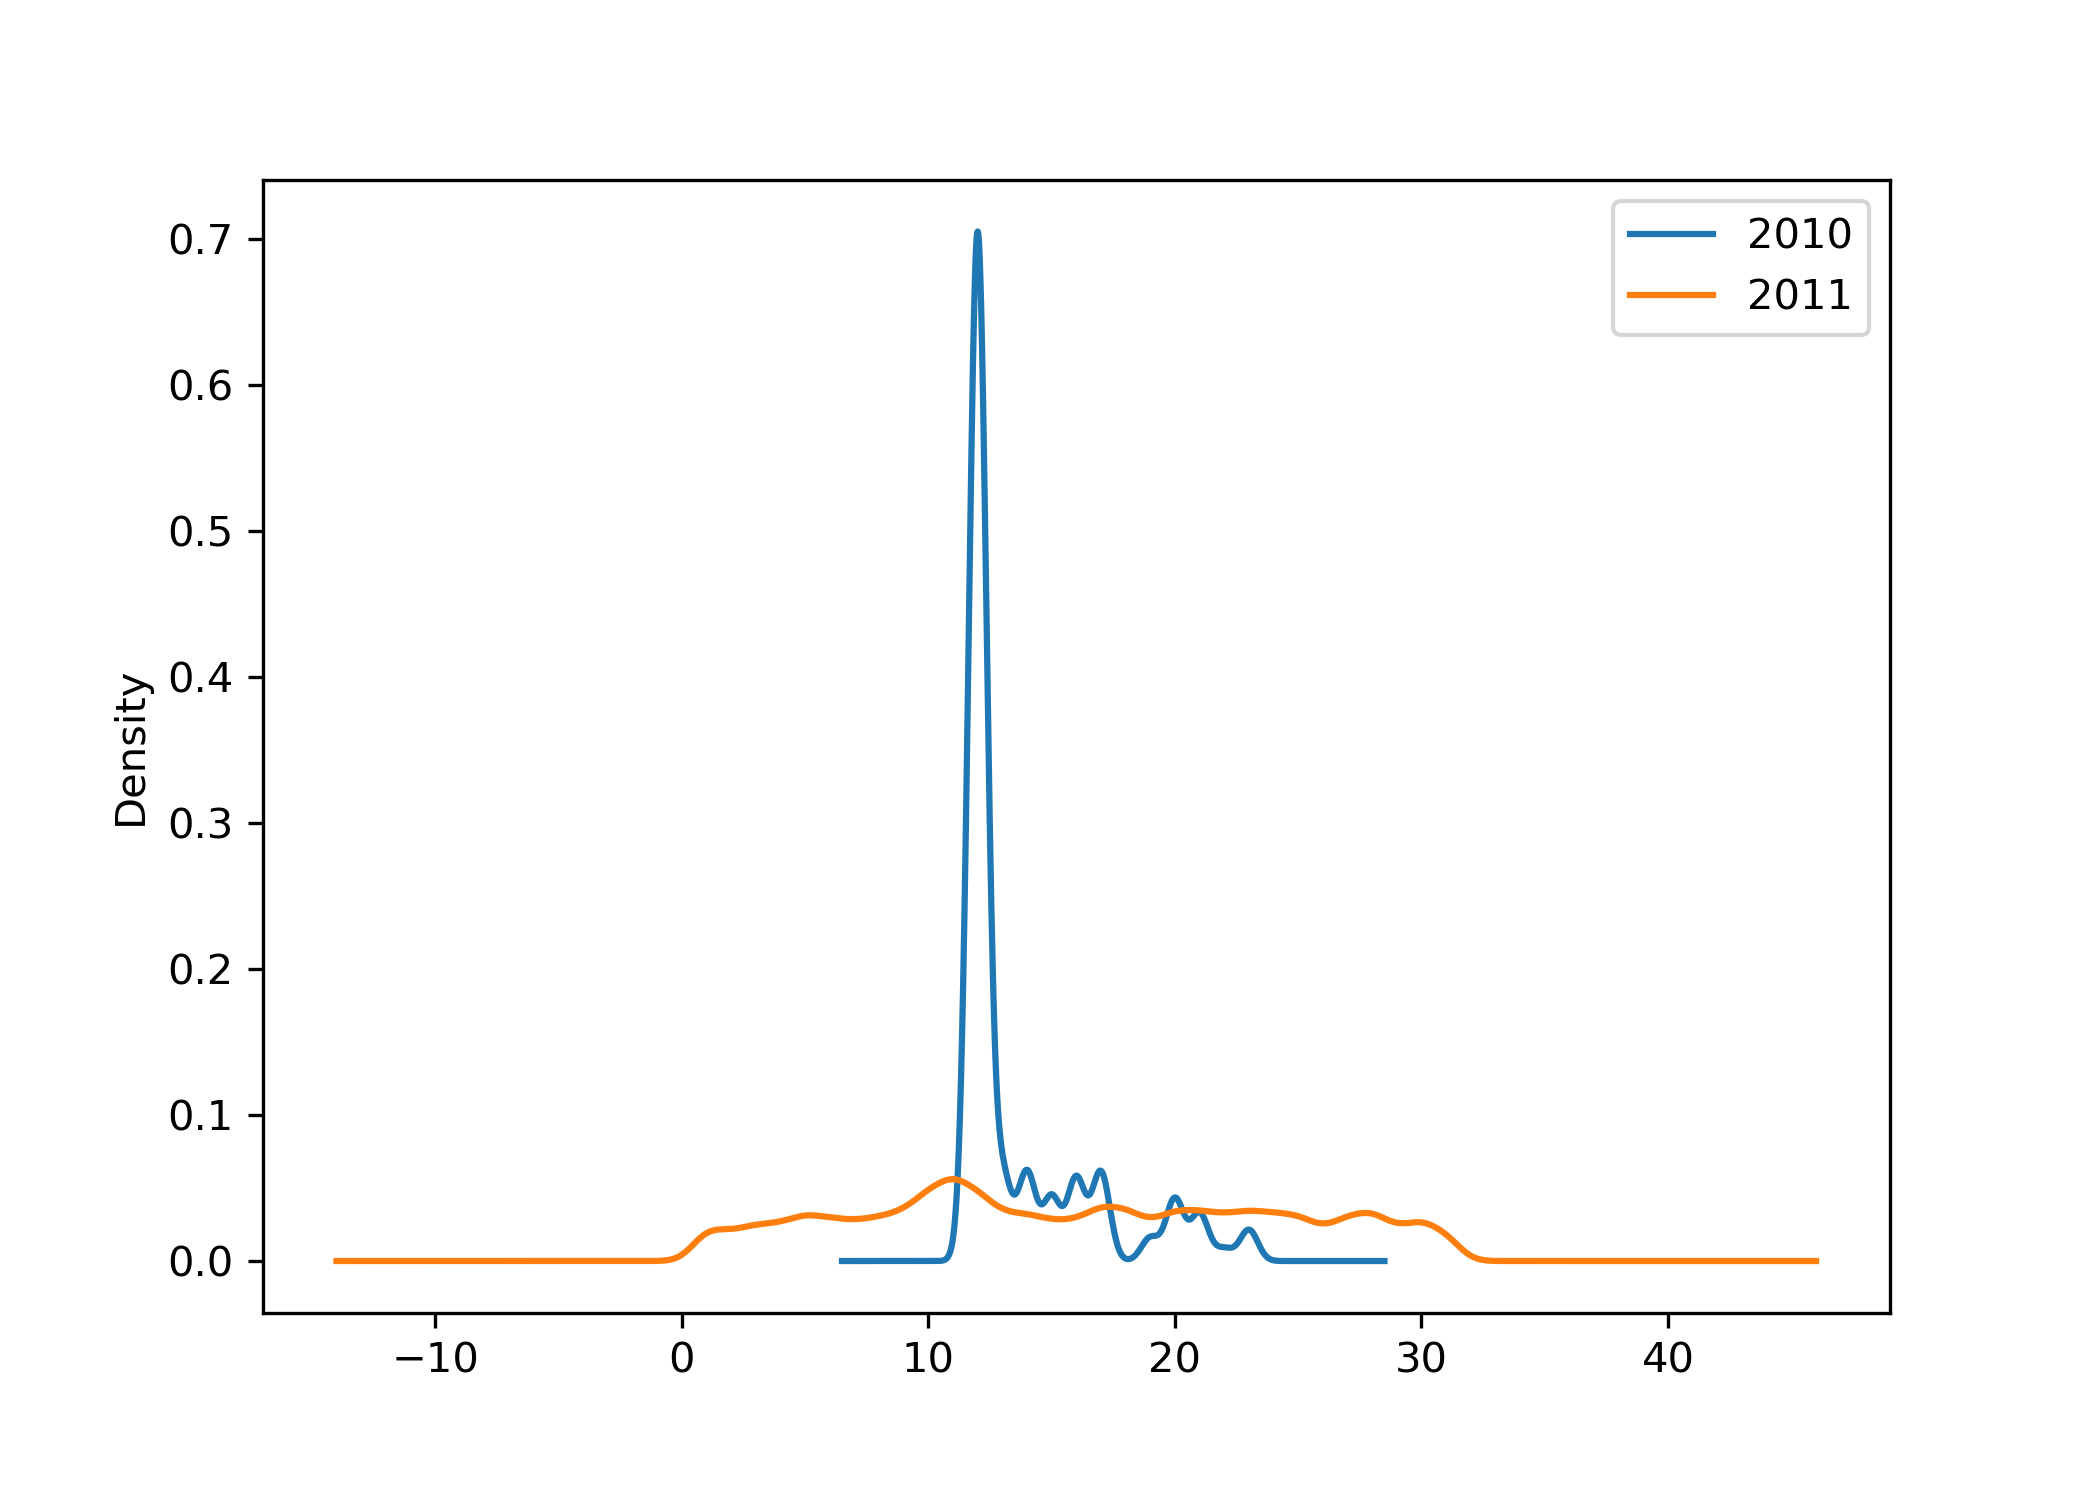
\includegraphics[width=.7\textwidth]{img/year_kde.png}
\caption{PDF by year}
\label{fig:year_kde}
\end{subfigure}
\begin{subfigure}{.33\textwidth}
\centering
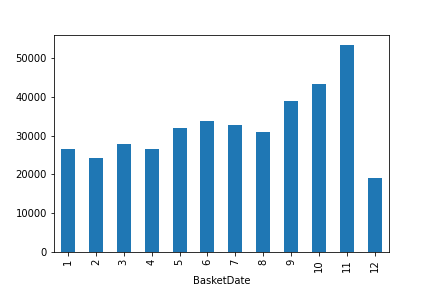
\includegraphics[width=.7\textwidth]{img/month_bar.png}
\caption{PDF by month}
\label{fig:month_bar}
\end{subfigure}
\begin{subfigure}{.33\textwidth}
\centering
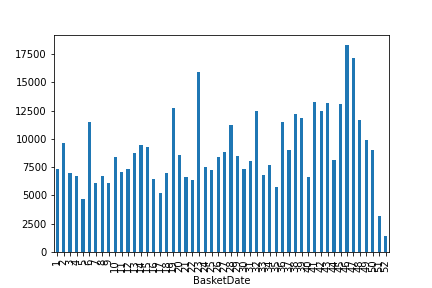
\includegraphics[width=.7\textwidth]{img/week_bar.png}
\caption{PDF by week}
\label{fig:week_bar}
\end{subfigure}
\begin{subfigure}{.33\textwidth}
\centering
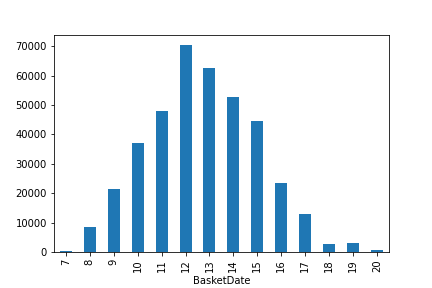
\includegraphics[width=.7\textwidth]{img/hour_bar.png}
\caption{PDF by hour}
\label{fig:hour_bar}
\end{subfigure}
\caption{BasketDate distributions}
\end{figure}

From the Figure \ref{fig:year_bar}, we can see that the attribute is highly unbalanced; in fact, we have that almost all the records are related to transaction of the 2011, while the objects from 2010 are very few. Indeed, the rows of 2011 represent about the 93\% of the whole dataset.\\
Furthermore, from the Figure \ref{fig:year_kde}, that represents an estimation of the probability density function of \emph{BasketDate} divided by year, we can appreciate the two different distributions.\\
In fact, for the 2010, we have a very uneven plot, which indicates that the records are not uniformly distributed with respect to the days in a month. This because, for the majority of the months in 2010, there were registered only transactions from a single day, the 12th; this is the value for which the plot shows the peak.\\
On the other hand, the distribution for the 2011 is much more homogeneous, meaning that the transactions were registered for most days in the months of that year. Other interesting distributions are plotted in Figure \ref{fig:month_bar}, \ref{fig:week_bar} and \ref{fig:hour_bar}. In the first one, we can see that the last weeks of the year are the one with more purchases; that is consistent with our expectations, since those are the weeks closest to Christmas time, that typically represents a great period of shopping. This thesis is supported also from the second one, in which we can see that December is the month with the most purchases. The third one is focused instead on the hours in a day; we found that, unsurprisingly, the most popular hourly is lunchtime.

\begin{figure}[!h]
\begin{subfigure}{.5\textwidth}
\centering
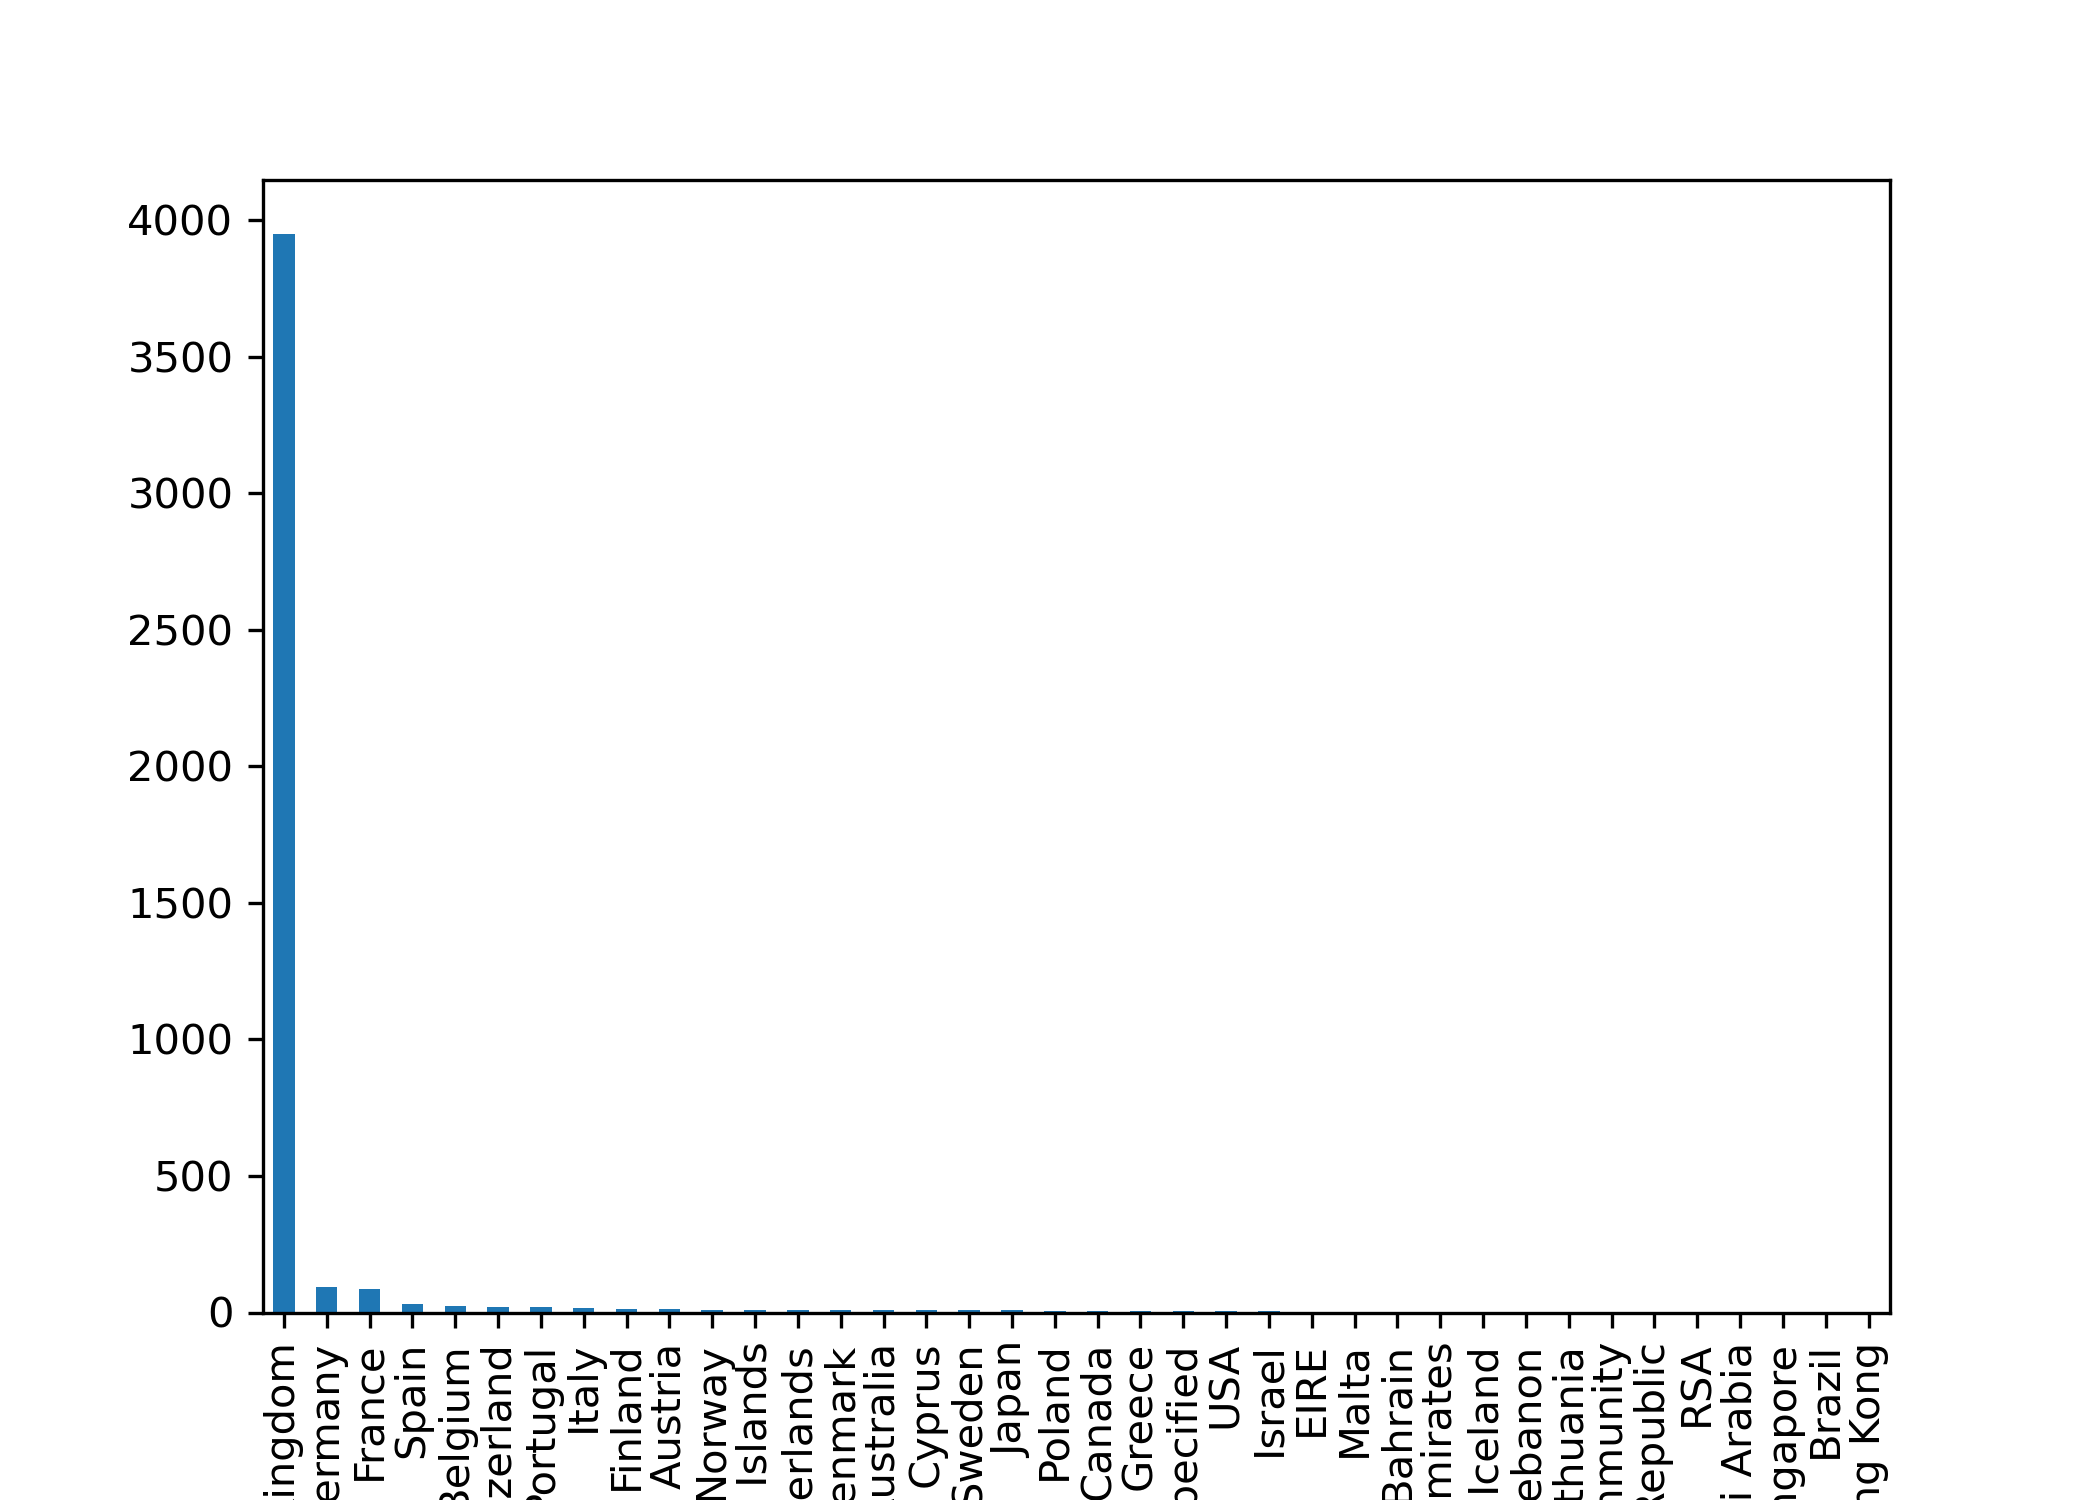
\includegraphics[width=.93\textwidth]{img/orders_country_bar.png}
\caption{}
\label{fig:orders_country_bar}
\end{subfigure}
\begin{subfigure}{.5\textwidth}
\centering
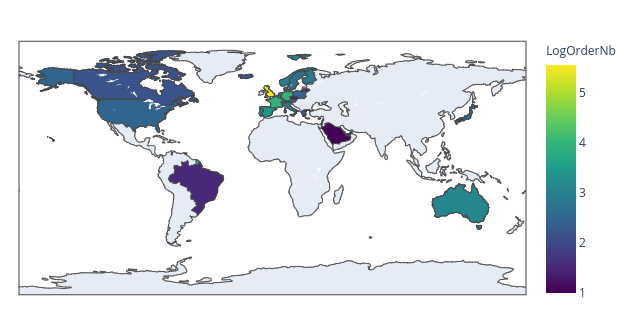
\includegraphics[width=.93\textwidth]{img/orders_country.png}
\caption{}
\label{fig:orders_country}
\end{subfigure}
\caption{CustomerCountry distributions}
\end{figure}

In Figure \ref{fig:orders_country_bar} and \ref{fig:orders_country}, we can see the distribution of the \emph{CustomerID} with respect to the country; from the plot, it is clear that the most frequent country is the \emph{United Kingdom}, that is present in about the 90\% of the rows.

\begin{wrapfigure}{r}{.5\textwidth}
\centering
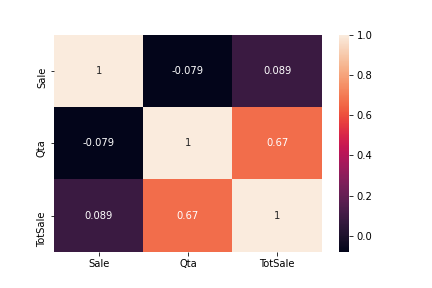
\includegraphics[width=0.49\textwidth]{img/dataset_corr.png}
\caption{Correlation Matrix}
\label{fig:dataset_corr}
\end{wrapfigure}

Finally, we see some informations about the correlation of the attributes, to see if some of them are redundant.\\
From the Figure \ref{fig:dataset_corr}, we can see that almost all the attributes are uncorrelated, except for \emph{TotSale}, that shows ah high correlation with \emph{Qta}; that follows what we expected, since \emph{TotSale} is, by construction, dependent on \emph{Qta}. So, we conclude that all the original columns are independent, and so we don't need to perform any further manipulation.
